\documentclass{tudelft-report}

%% Set up the bibliography
\usepackage{biblatex}
\addbibresource{report.bib}

%% Additional packages and commands
\usepackage{parskip}
\setlist{itemsep=-2pt} % Reducing white space in lists slightly
\renewcommand{\deg}{\si{\degree}\xspace} % Use \deg easily, everywhere
\usepackage{tcolorbox}

%% ----------------------------------------------------------------------
%%    Begin of document + Frontmatter (Roman page numbering)
%% ----------------------------------------------------------------------

\begin{document}

\frontmatter

%% Define the main parameters
\title{\textbf{Laboratorio} \\ Extracción de características y bolsa de palabras visuales}
\author{Ingeniería Matemática}

\subject{Visión por Ordenador I} % Cover only
\affiliation{Universidad Pontificia Comillas, ICAI} % Cover only
\coverimage{figures/cover.jpg} % Aspect ratio of 2:3 (portrait) recommended
\definecolor{title}{HTML}{ffffff} % Color for cover title

\makecover

\begin{titlepage}

\begin{center}

\bigskip
\bigskip

%% Print the name of the author
{\makeatletter
\begin{tabular}{c}
    3º \@author \\\midrule
    Curso 2024/25
\end{tabular}
\makeatother}

\bigskip
\bigskip

%% Print the title
{\makeatletter
\largetitlestyle\fontsize{45}{45}\selectfont\@title
\makeatother}

%% Print the subtitle
{\makeatletter
\ifdefvoid{\@subtitle}{}{\bigskip\titlestyle\fontsize{20}{20}\selectfont\@subtitle}
\makeatother}

%% Print table with names; easily add columns if necessary or remove the table completely
% \setlength\extrarowheight{2pt}
% \begin{tabular}{c}
%     3º  \\\midrule
%     Curso 2024/25 \\
% \end{tabular}

\vfill

%% Print some more information at the bottom
\begin{tabular}{ll}
    \textbf{Profesor}: & \textbf{Email} \\
    Erik Velasco & evelasco@icai.comillas.edu \\
    Lionel Güitta & lglopez@icai.comillas.edu \\
    Daniel Pinilla & dpinilla@icai.comillas.edu \\
    Luis Arias & learias@icai.comillas.edu \\
    Rodrigo Sánchez & rsmolina@icai.comillas.edu \\ 
    Ignacio de Rodrigo & iderodrigo@comillas.edu \\
\end{tabular}

\bigskip
\bigskip

%% Add a source and description for the cover and optional attribution for the template
\begin{tabular}{p{15mm}p{10cm}}
    Cover: & Canadarm 2 Robotic Arm Grapples SpaceX Dragon by NASA under CC BY-NC 2.0 (Modified) \\
    % Feel free to remove the following attribution, it is not required - still appreciated :-)
    % Style: & TU Delft Report Style, with modifications by Daan Zwaneveld
\end{tabular}
\vspace{10mm}

\end{center}

%% Insert the TU Delft logo at the bottom of the page
\begin{tikzpicture}[remember picture, overlay]
    \node[above=10mm] at (current page.south) {%
        
\includegraphics[scale=0.15]{figures/logo-color}
    };
\end{tikzpicture}

\end{titlepage}

%\chapter*{Preface}
\addcontentsline{toc}{chapter}{Preface}

\emph{A preface...}

\begin{flushright}
{\makeatletter\itshape
    \@author \\
    Delft, \monthname{} \the\year{}
\makeatother}
\end{flushright}

%\chapter*{Summary}
\addcontentsline{toc}{chapter}{Summary}

\emph{A summary...}


\tableofcontents
%\listoffigures
%\listoftables

%\chapter*{Nomenclature}
\addcontentsline{toc}{chapter}{Nomenclature}

\emph{If a nomenclature is required, a simple template can be found below for convenience. Feel free to use, adapt or completely remove.}

\section*{Abbreviations}

\begin{longtable}{p{2.5cm}p{8cm}}
    \toprule
    Abbreviation & Definition \\
    \midrule\endhead % Add abbreviations alphabetically here:
    ISA & International Standard Atmosphere \\
    ... \\
    \bottomrule
\end{longtable}

\section*{Symbols}

\begin{longtable}{p{2.5cm}p{8cm}p{2.5cm}}
    \toprule
    Symbol & Definition & Unit \\
    \midrule\endhead % Add Latin symbols alphabetically here:
    $V$ & Velocity & [m/s] \\
    ... \\
    \midrule % Add Greek symbols alphabetically here:
    $\rho$ & Density & [kg/m$^3$] \\
    ... \\
    \bottomrule
\end{longtable}


%% ----------------------------------------------------------------------
%%    Mainmatter (Arabic page numbering)
%% ----------------------------------------------------------------------

\mainmatter

\chapter{Sesión 3: Extracción de características y bolsa de palabras visuales}
\label{chapter:introduction_ses_3}

\section{Materiales}

En esta práctica se trabajará con los siguientes recursos (puede encontrarlos en la sección de Moodle \textit{Laboratorio/Sesión 3}):

\begin{itemize}
    \item \textbf{lab\_3.ipynb}: notebook con el código que deberá completar.
    \item \textbf{data}: carpeta con imágenes para trabajar durante la práctica.
\end{itemize}

\section{Apartados de la práctica}

La Sesión 3 del laboratorio está dividida en los siguientes apartados:

\begin{itemize}
    \item Instalaciones: Instalación de librerías necesarias.
    \item Librerías: Importación de las librerías que se utilizan en la sesión. Se recomienda realizar la importación en una celda inicial para mantener la organización del Notebook.
    \item Apartado A: .
    \item Apartado B: .
    \item Apartado C: .
\end{itemize}

\section{Observaciones}

Aunque el guion de la práctica y los comentarios en Markdown del Notebook estén escritos en español, observe que todo aquello que aparece en las celdas de código está escrito en inglés. Es una buena práctica que todo su código esté escrito en inglés.

Aquellas partes del código que deberá completar están marcadas con la etiqueta \textbf{\texttt{TODO}}.

Es muy importante que trabaje consultando la documentación de OpenCV\footnote{\href{https://docs.opencv.org/4.x/index.html}{Documentación de OpenCV}: \url{https://docs.opencv.org/4.x/index.html}} para familiarizarse de cara al examen. Tenga en cuenta que en los exámenes no podrá utilizar herramientas de ayuda como Copilot.

\section{Qué va a aprender}

Al finalizar esta práctica, sabrá cómo 

\section{Evaluación}

La nota que obtenga en esta sesión de laboratorio será la misma que obtenga su pareja. Los apartados de la práctica serán evaluados como refleja la Tabla \ref{table:evaluacion}. Tenga en cuenta que en esta práctica puede obtener puntuación extra si realiza el Apartado dedicado a \textit{Operadores Morfológicos}

\begin{table}[h!]
    \centering
    \begin{tabular}{|c|c|c|}
    \hline
    \textbf{Tarea} & \textbf{Valor} & \textbf{Resultado} \\
    \hline
    Pregunta A.1 & 3.0 & \\
    \hline
    Pregunta A.2 & 1.0 & \\
    \hline
    Pregunta B.1 & 3.0 & \\
    \hline
    Pregunta B.2 & 3.0 & \\
    \hline
    Pregunta C.1 & 2.0 & \\
    \hline
    \textbf{Total} & \textbf{12.0} & \\
    \hline
    \end{tabular}
    \caption{Valoración de los apartados de la práctica.}
    \label{table:evaluacion}
\end{table}

\chapter{Apartado A: \textbf{Segmentación por color}}
\label{chapter:tarea_a}

En este apartado deberá segmentar los colores blancos y naranjas que aparecen en las imágenes disponibles en la carpeta \texttt{data}. Segmentar por colores es una técnica sencilla y útil en aplicaciones en las que se tiene un gran control sobre las condiciones de contorno: iluminación, tipo de objeto que se espera encontrar, color del fondo, etc. A continuación se añaden algunos comentarios para resolver paso a paso la tarea:

\section*{Tarea A.1: Carga de imágenes}
\phantomsection
\addcontentsline{toc}{section}{Tarea A.1: Carga de imágenes}

Para trabajar de forma eficiente, antes de empezar a procesar imágenes deberá definir algunos métodos auxiliares. El primero de ellos es un método que debe cargar imágenes de la carpeta \texttt{data}.

\section*{Tarea A.2: Visualización y guardado de imágenes}
\addcontentsline{toc}{section}{Tarea A.2: Visualización y guardado de imágenes}

De nuevo, estos métodos ya los utilizó en la 1ª sesión de laboratorio, así que aproveche este paso para afianzar conceptos. Defina los métodos para visualizar imágenes y guardarlas. Respete y utilice todos los argumentos que se proporcionan.

\section*{Tarea A.3: Cambio de espacio de color}
\addcontentsline{toc}{section}{Tarea A.3: Cambio de espacio de color}

Cambie el espacio de color de las imágenes (BGR) a uno donde la crominancia e intensidad estén separados (HSV). Puede interpretar este paso como un cambio de sistema de referencia (cartesiano a polar). De esta forma, le será más fácil discriminar los colores de interés. La Figura \ref{fig:color_spaces} \footnote{ \href{https://commons.wikimedia.org/wiki/File:RGB\_2\_HSV\_conversion\_with\_grid.ogg}{Imagen modificada de VerbaGleb, CC BY-SA 4.0} https://commons.wikimedia.org/wiki/File:RGB\_2\_HSV\_conversion\_with\_grid.ogg} muestra los espacios de colores con los que trabajará.

Para cambiar el espacio de color de sus imágenes, puede utilizar el método \texttt{cv2.cvtColor()} de OpenCV. Tenga en cuenta que OpenCV cuenta con una gran cantidad de espacios de color, visite la documentación. \footnote{ \href{https://docs.opencv.org/3.4/d8/d01/group\_\_imgproc\_\_color\_\_conversions.html}{Espacios de color de OpenCV} https://docs.opencv.org/3.4/d8/d01/group\_\_imgproc\_\_color\_\_conversions.html}



\begin{figure}[h]
    \centering
    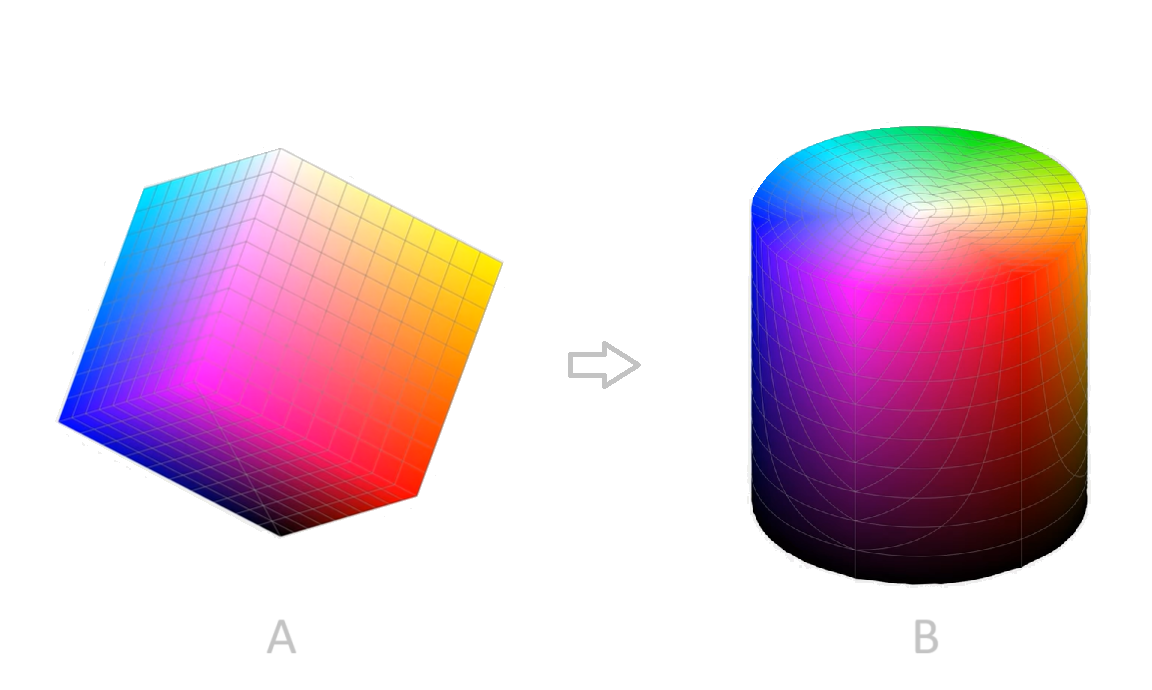
\includegraphics[width=0.5\textwidth]{Lab_2/template/figures/color_spaces.png}
    \caption{Espacios de color utilizados. Gráfico A: BGR (atención con el orden de canales en OpenCV) y Gráfico B: HSV.}
    
    \label{fig:color_spaces}
\end{figure}

\section*{Tarea A.4: Segmentación de las partes naranjas}
\addcontentsline{toc}{section}{Tarea A.4: Segmentación de las partes naranjas}

Genere una máscara para cada imagen y realice una segmentación con ella. Una máscara es una imagen binaria (blanca y/o negro) donde los píxeles de interés aparecen en blanco, mientras que los píxeles que no son de interés aparecen en negro. Segmentar implica multiplicar la imagen original con la máscara. Así se obtienen los píxeles de interés de la imagen original.

Para obtener las máscaras y segmentar la imagen, puede utilizar respectivamente los métodos \texttt{cv2.inRange()} y \texttt{cv2.bitwise\_and()} de OpenCV. Por otro lado, en este paso se facilitan los rangos de color naranja:

\begin{tcolorbox}[colback=gray!85, coltext=white, colframe=white, fonttitle=\bfseries, title=Important Note, boxrule=0.5mm]
\texttt{light\_orange = (1, 190, 200)}\\
\texttt{dark\_orange = (255, 255, 255)}
\end{tcolorbox}

Para confirmar que está obteniendo los resultados adecuados, muestre una de las imágenes iniciales, su máscara y la imagen segmentada.


\begin{figure}[h]
    \centering
    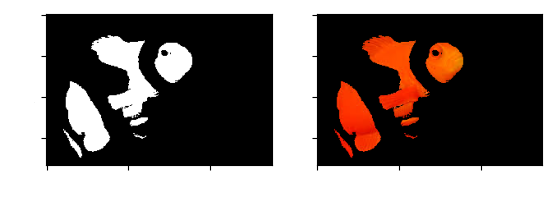
\includegraphics[width=0.5\textwidth]{Lab_2/template/figures/orange.png}
    \caption{Máscara y segmentación de colores naranjas.}
    \label{fig:orange_mask}
\end{figure}

\section*{Tarea A.5: Segmentación de las partes blancas}
\addcontentsline{toc}{section}{Tarea A.5: Segmentación de las partes blancas}

En este paso deberá repetir un proceso similar al anterior, pero centrándose en los tonos blancos. Explore el rango de valores necesarios para segmentar los colores blancos de las imágenes. Para ello, juegue con los valores de H, S y V en la interfaz que se le proporciona.

De nuevo, para confirmar que está obteniendo los resultados adecuados, muestre la máscara y la imagen segmentada.

\begin{figure}[h]
    \centering
    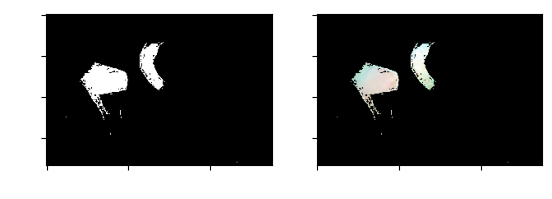
\includegraphics[width=0.5\textwidth]{Lab_2/template/figures/white.png}
    \caption{Máscara y segmentación de colores blancos.}
    \label{fig:whithe_mask}
\end{figure}

\section*{Tarea A.6: Combinación de máscaras}
\addcontentsline{toc}{section}{Tarea A.6: Combinación de máscaras}

Combine las máscaras de los colores naranja y blanco para cada imagen. Posteriormente, segmente cada imagen con la máscara que ha generado. Como resultado, conseguirá segmentar el cuerpo de los peces en el conjunto imágenes. Debería obtener resultados parecidos al ejemplo de la Figura \ref{fig:fish_output}.

Confirme que está obteniendo los resultados adecuados mostrando la máscara y la imagen segmentada.


\begin{figure}[h]
    \centering
    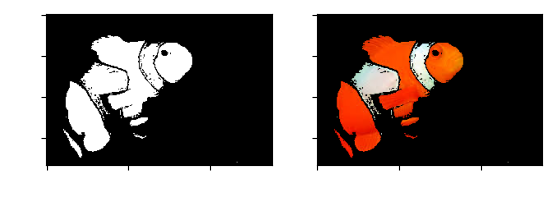
\includegraphics[width=0.5\textwidth]{Lab_2/template/figures/output.png}
    \caption{Máscara completa y segmentación del pez como combinación de colores blancos y naranjas.}
    \label{fig:fish_output}
\end{figure}


\section*{Tarea A.7: Guardado de imágenes}
\addcontentsline{toc}{section}{Tarea A.7: Guardado de imágenes}

Guarde las imágenes de interés como resultado de esta parte de la práctica.

\section*{Preguntas}
\addcontentsline{toc}{section}{Preguntas}

\vspace{5mm}
\begin{tcolorbox}[colback=gray!10, colframe=gray!30, coltitle=black, title=Pregunta A.1, halign=left]
Segmente por color el escudo de su equipo deportivo favorito: descompóngalo en al menos 2 colores. De igual forma que ha realizado en el ejercicio de clase, proporcione las máscaras binarias de cada color. Además, multiplique la máscara con la imagen original para visualizar solamente el color de interés. Por último indique el porcentaje que representa cada color sobre el total del escudo.
\end{tcolorbox}

\vspace{5mm}
\begin{tcolorbox}[colback=gray!10, colframe=gray!30, coltitle=black, title=Pregunta A.2, halign=left]
¿Qué ocurre cuando carga las imágenes con la librería \texttt{imageio} pero las visualiza con la librería \texttt{OpenCV}? Investigue qué puede estar pasando y cómo podría solucionarlo. Pista: cv2.cvtColor().
\end{tcolorbox}
\chapter{Apartado B: \textbf{Filtro Gaussiano y Detección de bordes: Sobel y Canny}}
\label{chapter:tarea_b}

En este apartado, trabajará con filtros para procesar imágenes. Los conceptos clave de este apartado son:

\begin{itemize}
    \item \textbf{Filtro o Kernel}: es una matriz $n x n$ que se desliza de forma ordenada por la imagen. Según sus valores, un filtro puede servir para difuminar una imagen, extraer sus bordes, etc.
    \item \textbf{Convolución}. Es una operación matemática que en visión por ordenador sirve para modificar una imagen. Toma los valores del kernel y los de la imagen en la posición $(i, j)$ para producir el valor del píxel $(i, j)$ de la nueva imagen. \footnote{\href{https://gitlab.com/brohrer/convolution-2d-animation/-/tree/main}{Ejemplos animados de convoluciones}: https://gitlab.com/brohrer/convolution-2d-animation/-/tree/main}
    \item \textbf{Imagen}: El elemento sobre el que se aplica la operación.
\end{itemize}

Trabajará en la definición de tres filtros: Gausiano, Sobel y Canny. Una vez definidos, deberá aplicar cada uno de los filtros sobre las imágenes de la carpeta \texttt{data}. A continuación se añaden algunos comentarios para resolver la tarea:

\section*{Tarea B.1: Implementación de filtro Gausiano}
\phantomsection
\addcontentsline{toc}{section}{Tarea B.1: Implementación de filtro Gausiano}

Para aplicar el filtro Gausiano, deberá tener cuenta los siguientes factores:

\begin{itemize}
    \item \textbf{Tamaño del filtro}. Como podrá comprobar en los argumentos de la función, el tamaño del filtro puede (o no) venir dado. Cuando el tamaño del filtro no se pase como argumento, deberá obtener sus dimensiones a partir del valor de $\sigma$. Puede dar por supuesto que el efecto del filtro Gausiano se considera extinto más allá de $\pm4\sigma$. Además, tenga en cuenta que se busca un filtro $n x n$ donde $n$ es impar. La Figura \ref{fig:kernel_size} ilustra cómo aumenta el tamaño del filtro (\textit{kernel size}, K) cuando aumenta $\sigma$.

    \begin{figure}[h]
    \centering
    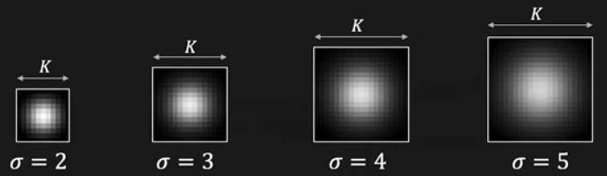
\includegraphics[width=0.6 \textwidth]{Lab_2/template/figures/kernel_size.png}
    \caption{Tamaño del kernel en función de $\sigma$.}
    \label{fig:kernel_size}
    \end{figure}

    Con las restricciones y condiciones mencionadas, deberá definir el tamaño del filtro de tal forma que se cumpla lo indicado en la Ecuación \ref{eq:kernel_size}:

    \begin{align}
     \text{shape} &= [L, L]\\
     L &= f(\sigma)
    \label{eq:kernel_size}
    \end{align}

    
    \item  \textbf{Coordenadas}. Con np.mgrid(), obtenga los valores de las coordenadas para $x$ e $y$ como dos arrays diferentes. Visite la documentación del método para visualizar un ejemplo de lo que se le pide.
    \item  \textbf{Fórmula}. Defina la fórmula del filtro Gausiano para cada elemento $(i, j)$ siguiendo la Ecuación \ref{eq:gausiano}.

    \begin{equation}
    G(i,j) = \frac{1}{\sigma \sqrt{2\pi}} e^{-\frac{1}{2} \left( \frac{i^2 + j^2}{\sigma^2} \right)}
    \label{eq:gausiano}
    \end{equation}

    \item  \textbf{Convolución}. Aplique sobre el argumento \texttt{img} la operación de convolución con el filtro que acaba de definir. Utilice el método de OpenCV \texttt{cv2.Filter2D()}.
\end{itemize}

\section*{Tarea B.2: Aplicación de filtro Gausiano}
\phantomsection
\addcontentsline{toc}{section}{Tarea B.2: Aplicación de filtro Gausiano}

Aplique el filtro que acaba de definir al conjunto de imágenes de la carpeta \texttt{data}. Defina las variables necesarias para llamar al método. Puede utilizar una \textit{list comprehension} para trabajar de forma eficiente. Como resultado de aplicar el filtro, debería obtener imágenes difuminadas o desenfocadas.

\section*{Tarea B.3: Implementación de filtro Sobel}
\phantomsection
\addcontentsline{toc}{section}{Tarea B.3: Implementación de filtro Sobel}

Para aplicar el filtro Sobel, deberá tener cuenta los siguientes factores:

\begin{itemize}
    \item \textbf{Imagen en escala de grises}. Trabaje con la imagen en escala de grises. Para ello, puede usar el método \texttt{cv2.cvtColor()} (que ya utilizó en la primera sesión de laboratorio).
    
    \item \textbf{Filtro Gausiano}. Utilice el método que ha definido anteriormente. Sea cuidadoso proporcionando cada argumento para que sea heredable (es decir, utilice variables como argumentos).
    
    \item \textbf{Bordes verticales}. Obtenga los bordes verticales utilizando el filtro dado (\texttt{filter}). De nuevo, utilice el método \texttt{cv2.Filter2D()}.
    \item \textbf{Transformación del filtro}. Transforme el filtro para obtener los bordes en la dirección ortogonal.
    \item \textbf{Bordes horizontales}. Con el filtro transformado, utilice de nuevo \texttt{cv2.Filter2D()} para obtener los bordes ortogonales.
    \item \textbf{Composición de bordes}. Obtenga los bordes de la imagen como una composición de los bordes detectados en cada dirección. Puede utilizar para ello \texttt{np.hypot()}.
    \item \textbf{Normalización}. Normalice el resultado anterior para evitar valores fuera de rango y ruidos.
    \item \textbf{Orientación}. Obtenga la orientación de los bordes con \texttt{np.arctan2()}.
\end{itemize}

\section*{Tarea B.4: Aplicación de filtro Sobel}
\phantomsection
\addcontentsline{toc}{section}{Tarea B.4: Aplicación de filtro Sobel}

Aplique el filtro que acaba de definir al conjunto de imágenes de la carpeta \texttt{data}. Defina las variables necesarias para llamar al método. Puede utilizar una \textit{list comprehension} para trabajar de forma eficiente. Como resultado de aplicar el filtro, debería obtener un resultado similar al de la Figura \ref{fig:edges}.

\begin{figure}[H]
    \centering
    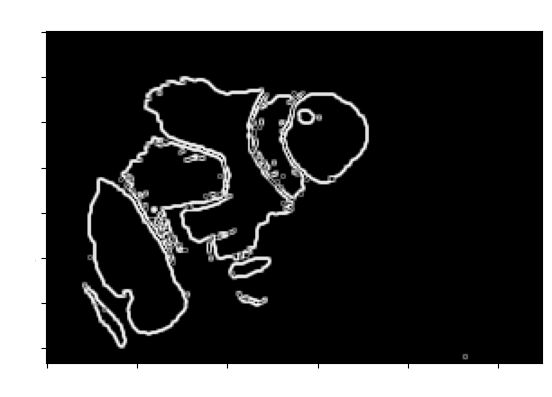
\includegraphics[width=0.3\textwidth]{Lab_2/template/figures/edges.png}
    \caption{Ejemplo de bordes detectados usando el filtro Sobel.}
    \label{fig:edges}
\end{figure}

\section*{Tarea B.5: Implementación de filtro Canny}
\phantomsection
\addcontentsline{toc}{section}{Tarea B.5: Implementación de filtro Canny}
El filtro Canny aporta un resultado más refinado para detectar bordes que el obtenido por Sobel. Para implementar el filtro Canny, deberá seguir los siguientes pasos:

\begin{itemize}
    \item \textbf{Filtro Sobel}. Realice una llamada al método del filtro Sobel que ha definido en los pasos anteriores. De nuevo,  sea cuidadoso proporcionando cada argumento para que sea heredable (es decir, utilice variables como argumentos).
    \item \textbf{Non Max Supresion}. Utilice el método \texttt{non\_max\_supression()} definido en el archivo \texttt{utils.py}. Inspeccione los argumentos que necesita utilizar este método para poder ejecutarlo de forma adecuada. Este método se encarga de refinar los bordes, devolviendo una imagen en escala de grises. 
\end{itemize}

\section*{Tarea B.6: Aplicación de filtro Canny}
\phantomsection
\addcontentsline{toc}{section}{Tarea B.6: Aplicación de filtro Canny}

Aplique el filtro que acaba de definir al conjunto de imágenes de la carpeta \texttt{data}. Defina las variables necesarias para llamar al método. Puede utilizar una \textit{list comprehension} para trabajar de forma eficiente. Como resultado de aplicar el filtro, debería obtener los bordes de las imágenes de forma similar a cuando aplicó el filtro Sobel.

\section*{Preguntas}
\addcontentsline{toc}{section}{Preguntas}

\vspace{5mm}
\begin{tcolorbox}[colback=gray!10, colframe=gray!30, coltitle=black, title=Pregunta B.1, halign=left]
Añada ruido a las imágenes de la carpeta \texttt{data}. Compare los resultados que obtiene al aplicar su filtro Sobel \textbf{con y sin filtro Gausiano}. Para añadir ruido, puede sumar a la imagen original una matriz de las dimensiones adecuadas. Puede utilizar \texttt{np.random.normal()}, pero tenga en cuenta que este proceso puede hacer que algunos valores de la imagen salgan del rango [0, 255] (tome las medidas necesarias para corregir esto).
\end{tcolorbox}

\vspace{5mm}
\begin{tcolorbox}[colback=gray!10, colframe=gray!30, coltitle=black, title=Pregunta B.2, halign=left]
Utilice la librería \texttt{scikit-image} y compare el efecto de los filtros Sobel, Canny y Prewitt sobre las imágenes de la carpeta \texttt{data}. ¿Qué diferencias observa entre los filtros? ¿Puede obtener alguna conclusión y/o patrón?
\end{tcolorbox}
\chapter{Apartado C: \textbf{Operadores morfológicos}}
\label{chapter:tarea_c}

Esta sección es completamente voluntaria y puede realizarla para mejorar su puntuación en la práctica.

\vspace{5mm}
\begin{tcolorbox}[colback=gray!10, colframe=gray!30, coltitle=black, title=Pregunta C.1, halign=left]
Implemente los operadores morfológicos dilatación y erosión. Utilice para ello un kernel de 3x3 con valores 255 (blanco) como structuring element. No olvide binarizar su imagen antes de aplicar los operadores morfológicos.
\end{tcolorbox}

%% Prevent urls running into margins in bibliography
\setcounter{biburlnumpenalty}{7000}
\setcounter{biburllcpenalty}{7000}
\setcounter{biburlucpenalty}{7000}

%% Add bibliography
% \printbibliography[heading=bibintoc,title=References]

%% ----------------------------------------------------------------------
%%    Appendix (Letters for chapters)
%% ----------------------------------------------------------------------

%\appendix

%\chapter{Source Code Example}
%\label{chapter:title}

\emph{Adding source code to your report/thesis is supported with the package {\normalfont\texttt{listings}}. An example can be found below. Files can be added using {\normalfont\texttt{\textbackslash lstinputlisting[language=<language>]\{<filename>\}}}.}

\begin{lstlisting}[language=Python]
"""
ISA Calculator: import the function, specify the height and it will return a
list in the following format: [Temperature,Density,Pressure,Speed of Sound].
Note that there is no check to see if the maximum altitude is reached.
"""

import math
g0 = 9.80665
R = 287.0
layer1 = [0, 288.15, 101325.0]
alt = [0,11000,20000,32000,47000,51000,71000,86000]
a = [-.0065,0,.0010,.0028,0,-.0028,-.0020]

def atmosphere(h):
    for i in range(0,len(alt)-1):
        if h >= alt[i]:
            layer0 = layer1[:]
            layer1[0] = min(h,alt[i+1])
            if a[i] != 0:
                layer1[1] = layer0[1] + a[i]*(layer1[0]-layer0[0])
                layer1[2] = layer0[2] * (layer1[1]/layer0[1])**(-g0/(a[i]*R))
            else:
                layer1[2] = layer0[2]*math.exp((-g0/(R*layer1[1]))*(layer1[0]-layer0[0]))
    return [layer1[1],layer1[2]/(R*layer1[1]),layer1[2],math.sqrt(1.4*R*layer1[1])]
\end{lstlisting}

%\chapter{Task Division Example}
%\label{chapter:title}

\emph{If a task division is required, a simple template can be found below for convenience. Feel free to use, adapt or completely remove.}

\begin{table}[htb]
    \setlength\extrarowheight{4pt}
    \centering
    \caption{Distribution of the workload}
    \label{tab:taskdivision}
    \begin{tabularx}{\textwidth}{lXX}
        \toprule
        & Task & Student Name(s) \\
        \midrule
        & Summary & \\
        Chapter 1 & Introduction &  \\
        Chapter 2 &  & \\
        Chapter 3 &  & \\
        Chapter * &  & \\
        Chapter * & Conclusion &  \\
        \midrule
        & Editors & \\
        & CAD and Figures & \\
        & Document Design and Layout & \\
        \bottomrule
    \end{tabularx}
\end{table}

%\input{appendix/appendix-c} % Create file to add

\end{document}
